% Класс документа с параметрами: кегль шрифта, шрифт с засечками для формул,
% соотношение сторон слайда
\documentclass[14pt,mathserif,aspectratio=43]{beamer}

% Кодировка файла
\usepackage[utf8]{inputenc}
% Переносы для русского языка
\usepackage[russian]{babel}

\usepackage{xcolor}
% Цвет логотипа лаборатории
\definecolor{lab-blue}{RGB}{30,97,182}
% Ищется в яндексе по запросу «травяной цвет»
\definecolor{grass}{RGB}{93,161,48}

\usepackage[T1]{fontenc}
% Шрифт для формул
\usepackage[bitstream-charter]{mathdesign}

% Математические символы
\usepackage{amsmath}

% Перечёркивание текста
\usepackage{ulem}

% Основной цвета beamer'а (по умолчанию — синий)
\setbeamercolor{structure}{fg=black}

% Путь к картинкам
\graphicspath{{images/}}

% Нумерация слайдов
\setbeamertemplate{footline}{%
\raisebox{7pt}{\makebox[\paperwidth]{%
\hfill\makebox[10pt]{\scriptsize\textcolor{gray}{\insertframenumber~~~~}}}}}

% Начинать нумерацию слайдов не с титульного слайда
% \let\otp\titlepage
% \renewcommand{\titlepage}{\otp\addtocounter{framenumber}{-1}}

% Сноска без номера
\newcommand\articlenote[1]{%
  \begingroup%
  \renewcommand\thefootnote{}\footnote{#1}%
  \addtocounter{footnote}{-1}%
  \endgroup%
}

% Убрать навигацию beamer'а по умолчанию
\beamertemplatenavigationsymbolsempty

% Параметры для создания титульной страницы
\title{Предсказание цен на отели на основе данных с сайта бронирования\vspace{-1em}}
\author{Выполнили:\\Богомолов Эмиль, \\ Лютов Владимир.}
\usepackage{epstopdf}


% Время
\date{\small{18 декабря 2017}}

\begin{document}

%-------------------------------------------------------------------------------
\begin{frame}[plain]
    \titlepage
 \end{frame}

%-------------------------------------------------------------------------------
\begin{frame}[label=target]{Цель проекта}

    \textcolor{lab-blue}{Получение данных}

    Мы добыли данные с ресурса Booking.com по ценам на отели о. Майорка

    \textcolor{lab-blue}{Цель}
    
    Предсказание оптимальной цены номера. Чтобы отелю максимизировать прибыль, а туристу не переплачивать.
    
    \hyperlink{sad}{\beamerbutton{Спрос и предложение}}
    
\end{frame}

%-------------------------------------------------------------------------------
\begin{frame}{Получение данных}

    \begin{columns}[t]
    \column{.5\textwidth}
    \centering
    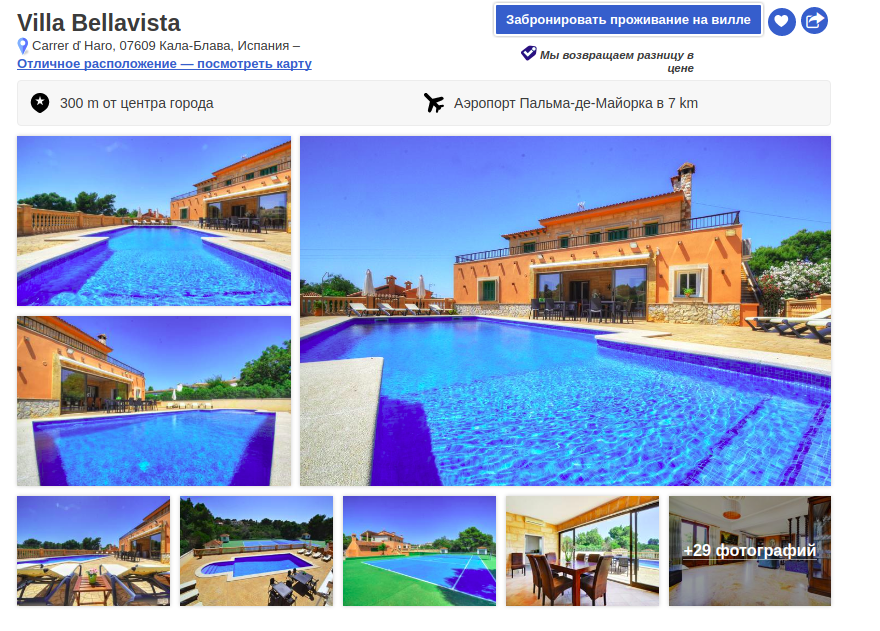
\includegraphics[width=5cm,height=3.5cm]{villa.png}\\
    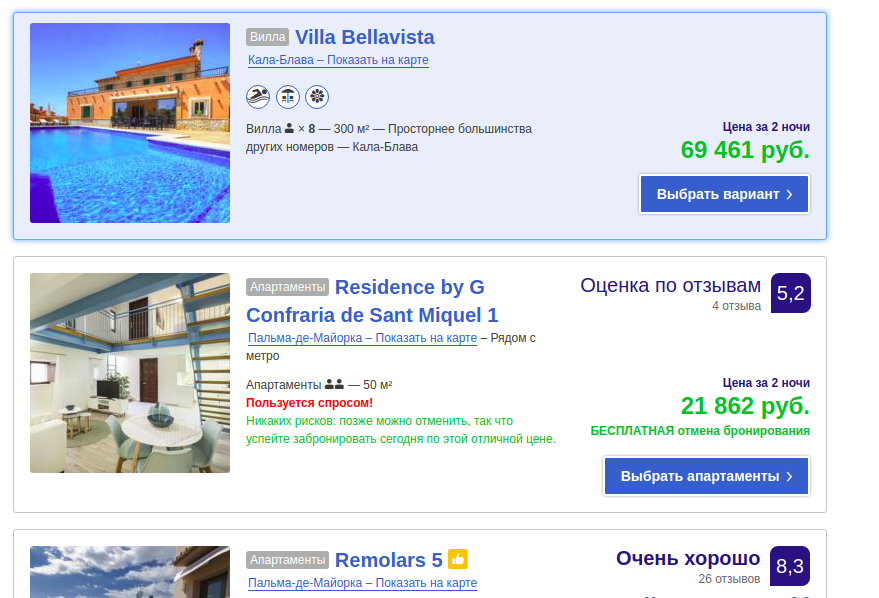
\includegraphics[width=5cm,height=3.5cm]{prices.png}\\
    \column{.5\textwidth}
    \centering
    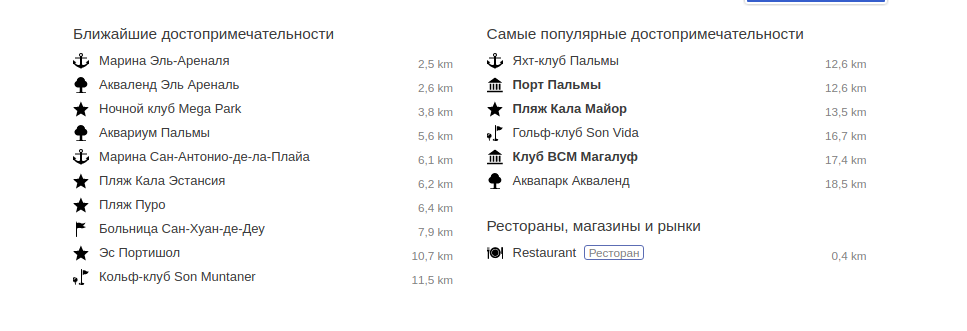
\includegraphics[width=5cm,height=3cm]{sights.png}\\
    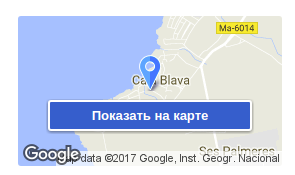
\includegraphics[width=5cm,height=3cm]{map.png}
\end{columns}

\end{frame}

%-------------------------------------------------------------------------------
\begin{frame}{Данные}
    Следующая информация была получена:
    \begin{itemize}
        \item цены на номера, виллы и общие комнаты,
        \item количество спальных мест в помещении и площадь,
        \item расстояния до ориентиров поблизости и их количество,
        \item рейтинг отеля и количество проголосовавших,
        \item географические координаты отеля.
    \end{itemize}

\end{frame}

%-------------------------------------------------------------------------------

\begin{frame}{Пред-обработка}

    \textcolor{lab-blue}{Удалить выбросы}
    
    \begin{center}
        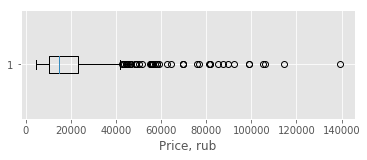
\includegraphics[width=0.8\textwidth]{boxplot.png}
    \end{center}

    \textcolor{lab-blue}{Описание номера}
    
    Поиск по ключевым словам \\ % 'Двухместный', 'кроватями', 'кроватью', 'Апартаменты', 'Вилла', 'Номер-студио', 'Дом', 'Люкс' \\
    Обработка с помощью one-hot или счетчиков % (но не фортануло)

    \textcolor{lab-blue}{Все остальные данные}
    
    Стандартная пред-обработка

\end{frame}

%-------------------------------------------------------------------------------

\begin{frame}{Рассматривали модели}

    \begin{itemize}
        \item Lasso, Ridge
        \item SVR; Kernels: Linear, Poly, RBF % (=KNN)
        \item Random Forest
        \item Gradient Boosting
        \item KNN
    \end{itemize}
    
    \begin{center}
        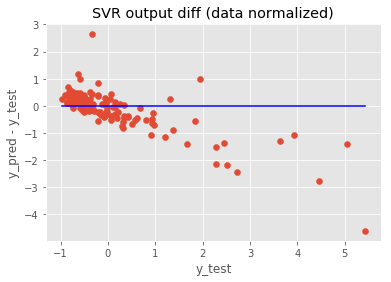
\includegraphics[width=0.5\textwidth]{loss.png}
    \end{center}

\end{frame}

%-------------------------------------------------------------------------------

\begin{frame}{Что не сработало}

    \begin{itemize}
        \item Ключевые слова
        \item Уменьшение размерности, чтобы избежать переобучения
        \item Расстояние до достопримечательностей и берега
    \end{itemize}
    
    \begin{center}
        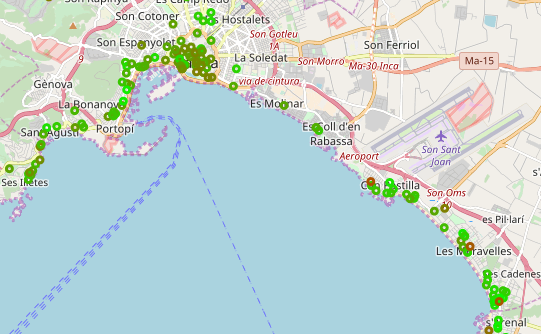
\includegraphics[width=0.75\textwidth]{map_prices.png}
    \end{center}

\end{frame}

%-------------------------------------------------------------------------------

\begin{frame}[label=model]{Модель и критерий качества}

    \begin{itemize}
        \item SVR with RBF kernel
        \item Tuning parameters \hyperlink{learning}{\beamerbutton{learning}}
        \item Explained variation: 55 \% \hyperlink{ev}{\beamerbutton{define}}
    \end{itemize}
    
    \begin{center}
        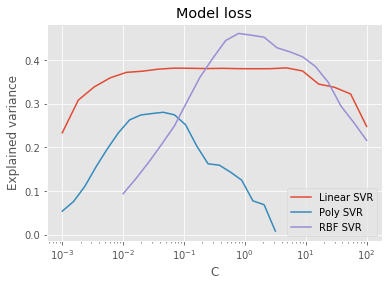
\includegraphics[width=0.8\textwidth]{svr_loss.png}
    \end{center}
    
\end{frame}

%-------------------------------------------------------------------------------

\begin{frame}{Выводы}

    \begin{itemize}
        \item Получили данные с сайта booking.com
        \item Построили линейную модель, которая предсказывает 55 \% дисперсии цены
        \item Более сложные модели показали низкие результаты % Возможно, для их обучения нужно агрегировать данные по нескольким регионам 
    \end{itemize}

\end{frame}

%-------------------------------------------------------------------------------

\begin{frame}[label=learning]{Обучение}

    \begin{itemize}
        \item Пред-обработка
        \item Данные разбивались на train и test set 8/2
        \item Для проверки качества использовался усредненный Explained Variation с использованием KFold на train set
        \item Для тюнинга параметров использовался Grid Search CV
    \end{itemize}
    
    \hyperlink{model}{\beamerbutton{Назад}}

\end{frame}

%-------------------------------------------------------------------------------

\begin{frame}[label=ev]{Explained variation}

    $$
        \texttt{explained\_{}variance}(y, \hat{y}) = 1 - \frac{Var\{ y - \hat{y}\}}{Var\{y\}}
    $$
    
    The best possible score is 1.0, lower values are worse.
    
    \hyperlink{model}{\beamerbutton{Назад}}

\end{frame}

%-------------------------------------------------------------------------------

\begin{frame}[label=sad]{Supply and demand}

    \begin{center}
        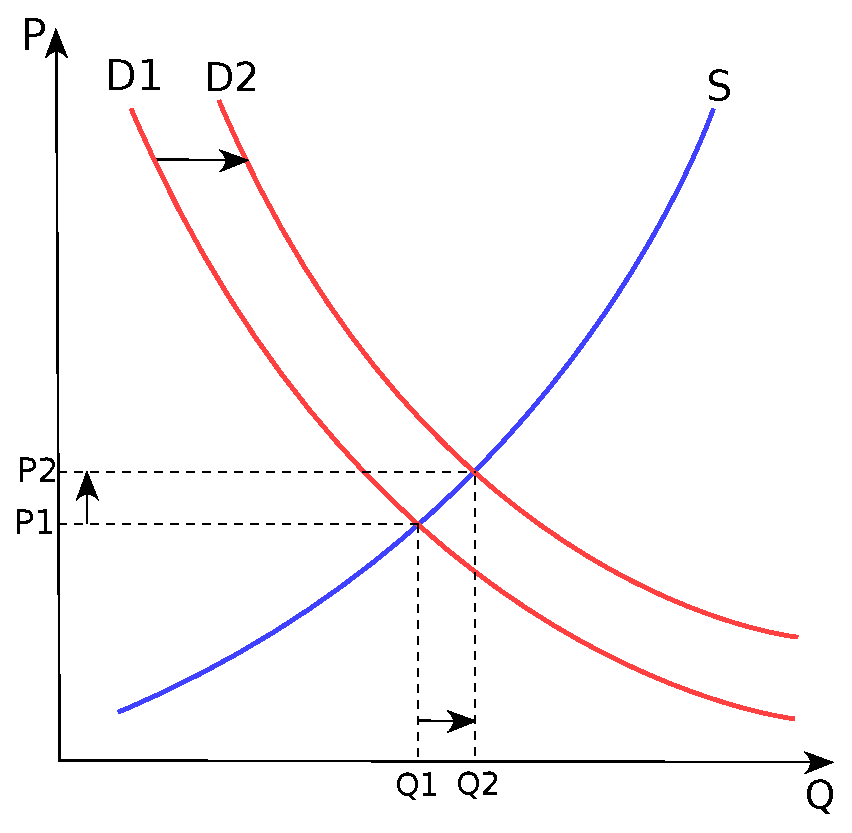
\includegraphics[width=0.5\textwidth]{Supply-and-demand.eps} \\
        \footnotesize{The price P of a product is determined by a balance between production at each price (supply S) and the desires of those with purchasing power at each price (demand D). The diagram shows a positive shift in demand from D1 to D2, resulting in an increase in price (P) and quantity sold (Q) of the product.}
    \end{center}
    
    \hyperlink{target}{\beamerbutton{Назад}}

\end{frame}

%-------------------------------------------------------------------------------


\end{document}

